\begin{refsection}
  \begin{frame}{Image Classification: Overview}
    \begin{figure}
      \centering
      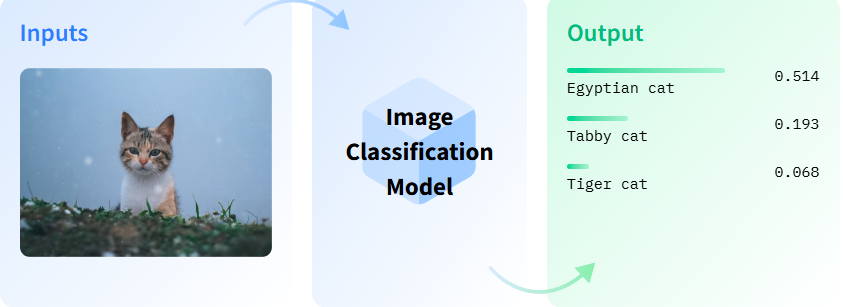
\includegraphics[height=0.6\textheight]{image_classification_idea.png}
      {\scriptsize Overview of image classification.\\\ \textit{Image source: Hugging Face tutorial}}
    \end{figure}
    \bottomleftrefs
  \end{frame}
\end{refsection}

\begin{refsection}
  \begin{frame}{Background: AlexNet Architecture}
    \begin{figure}
      \centering
      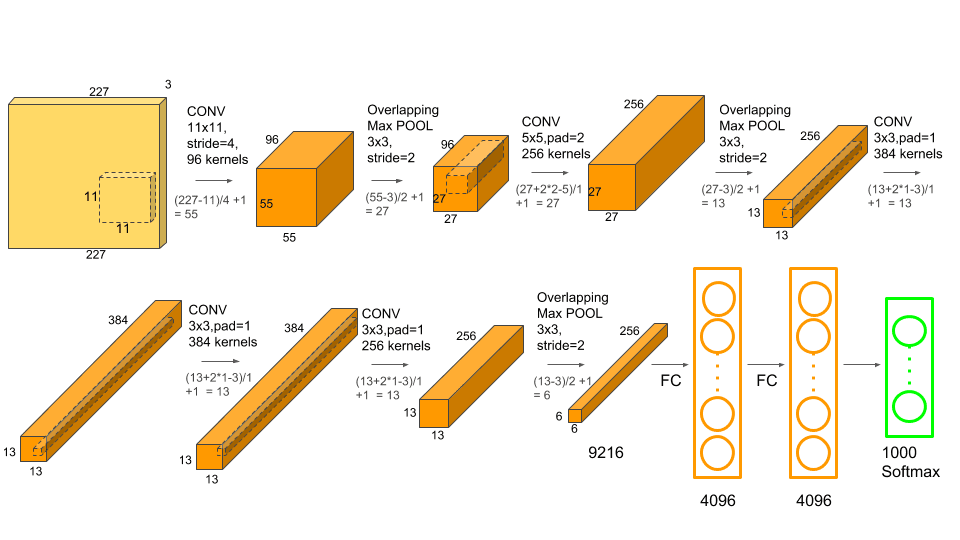
\includegraphics[width=0.8\linewidth]{alexnet.png}
      \caption[]{\scriptsize Architecture of AlexNet~\parencite{krizhevskyImageNetClassificationDeep2012}.~\textit{Image source: Web}}
    \end{figure}
    \bottomleftrefs
  \end{frame}
\end{refsection}

\begin{refsection}
  \begin{frame}{AlexNet: ILSVRC-2012 Results}
    \begin{itemize}
      \item AlexNet~\parencite{krizhevskyImageNetClassificationDeep2012} achieved a winning top-5 test error rate of \textbf{15.3\%} in the ILSVRC-2012 competition, compared to 26.2\% by the second-best entry.
    \end{itemize}
    \vspace{0.5em}
    \begin{table}[h]
      \centering
      \begin{tabular}{|l|c|c|c|}
      \hline
      \textbf{Model} & \textbf{Top-1 (val)} & \textbf{Top-5 (val)} & \textbf{Top-5 (test)} \\
      \hline
      \textit{SIFT + FVs} & --- & --- & 26.2\% \\
      1 CNN & 40.7\% & 18.2\% & --- \\
      5 CNNs & 38.1\% & 16.4\% & \textbf{16.4\%} \\
      1 CNN* & 39.0\% & 16.6\% & --- \\
      7 CNNs* & 36.7\% & 15.4\% & \textbf{15.3\%} \\
      \hline
      \end{tabular}
      \caption{\scriptsize Comparison of error rates on ILSVRC-2012 validation and test sets. \textit{Italics}: best results by others. *: Models pre-trained on ImageNet 2011 Fall release.}
    \end{table}
    \bottomleftrefs
  \end{frame}
\end{refsection}
  

\begin{refsection}
  \begin{frame}{Background: Image Classification with Deep Learning}
    \begin{figure}
      \centering
      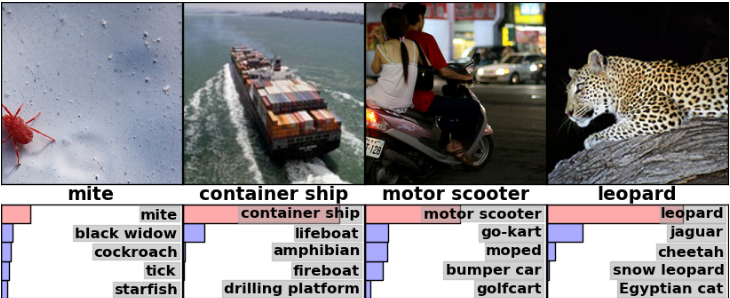
\includegraphics[width=1.0\linewidth]{imagenet2.png}
      \caption[]{\scriptsize AlexNet on ILSVRC-2010~\parencite{imagenet2010challenge}.}
    \end{figure}
    \bottomleftrefs
  \end{frame}
\end{refsection}

\begin{frame}{Background: ResNet (2016)}
  \begin{itemize}
    \item Key innovation: residual (skip) connections.
    \item Enabled extremely deep networks (up to 152 layers).
    \item Achieved state-of-the-art performance in ILSVRC-2015.
  \end{itemize}
  \begin{figure}
    \centering
    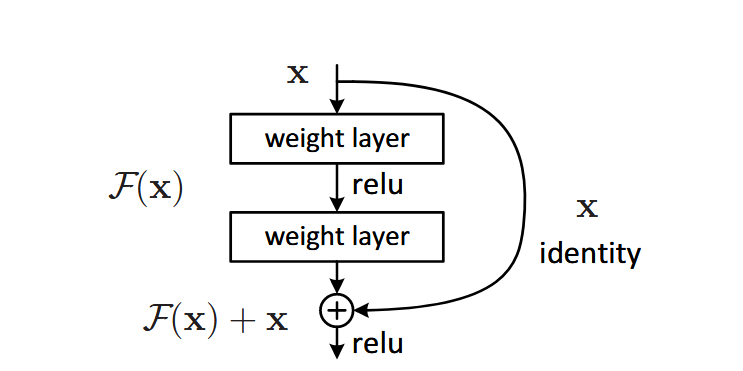
\includegraphics[width=0.7\linewidth]{resnet.png}
    \caption{\scriptsize ResNet block with identity mapping~\parencite{heDeepResidualLearning2016}.}
  \end{figure}
\end{frame}

\begin{frame}{Transformers for Image Classification}
  \begin{itemize}
    \item \textbf{Vision Transformer (ViT, 2021):} Applies transformer models from NLP to image patches.
    % \item \textbf{Swin Transformer (2021):} A hierarchical vision transformer using shifted windows.
    % \item \textbf{CLIP, MAE, CoCa:} Leverage massive datasets, contrastive learning, and self-supervised methods.
  \end{itemize}
  \begin{figure}
    \centering
    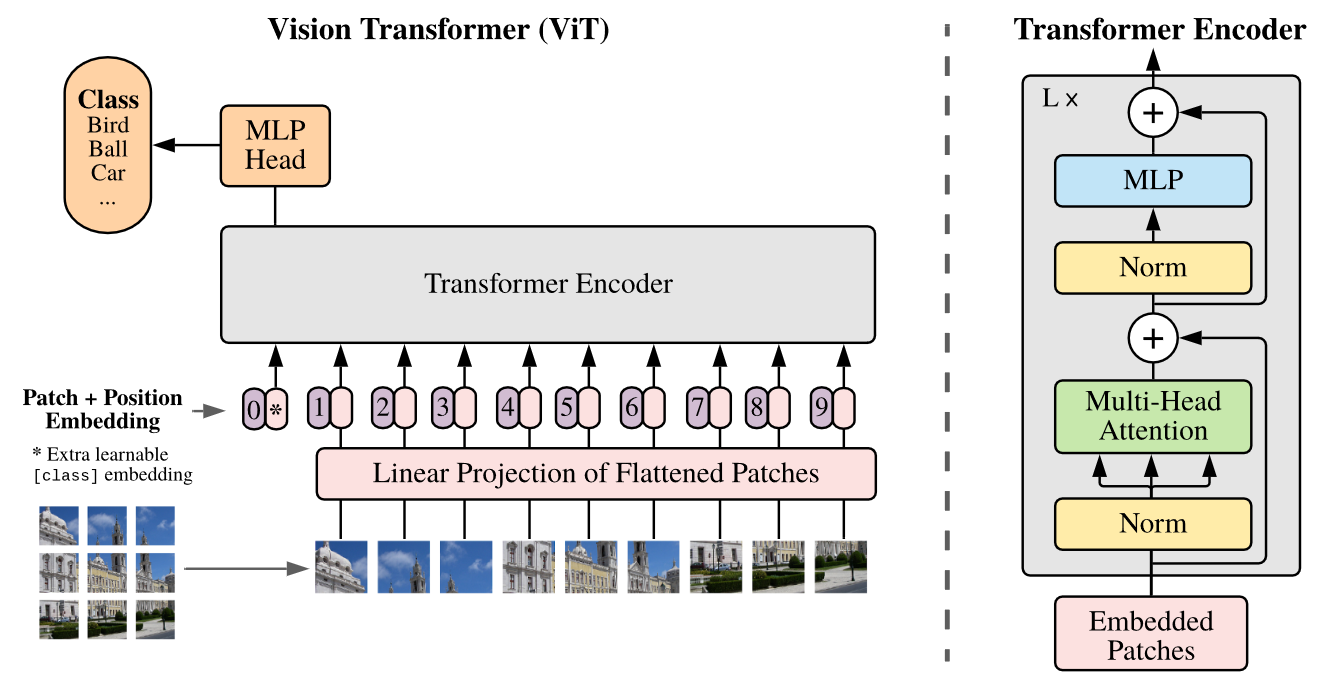
\includegraphics[width=0.7\linewidth]{vit.png}
    \caption{\scriptsize Vision Transformer overview~\parencite{dosovitskiyImageWorth16x162020}.}
  \end{figure}
\end{frame}


% \begin{refsection}
%   \begin{frame}{Architecture Evolution of Image Classification}
%     \begin{minipage}{0.48\linewidth}
%       {\small
%       \begin{itemize}
%         % \item \textbf{2012: AlexNet} \\
%         % \parencite{krizhevskyImageNetClassificationDeep2012}
%         % \item \textbf{2016: ResNet} \\
%         % \parencite{heDeepResidualLearning2016}
%         \item \textbf{2012: AlexNet}, \textbf{2016: ResNet} \\
%         \item \textbf{2021: ViT} \\
%         \parencite{dosovitskiyImageWorth16x162020}
%         \item \textbf{2021: Swin Transformer} \\
%         \parencite{liuSwinTransformerHierarchical2021}
%         \item \textbf{2021: CLIP-ViT} \\
%         \parencite{radfordLearningTransferableVisual2021}
%         \item \textbf{2022: MAE-ViT} \\
%         \parencite{heMaskedAutoencodersAre2022}
%         \item \textbf{2022: CoCa-ViT} \\
%         \parencite{yuCoCaContrastiveCaptioners2022}
%       \end{itemize}
%       }
%     \end{minipage}%
%     \hfill
%     % \begin{minipage}{0.48\linewidth}
%     %   \centering
%     %   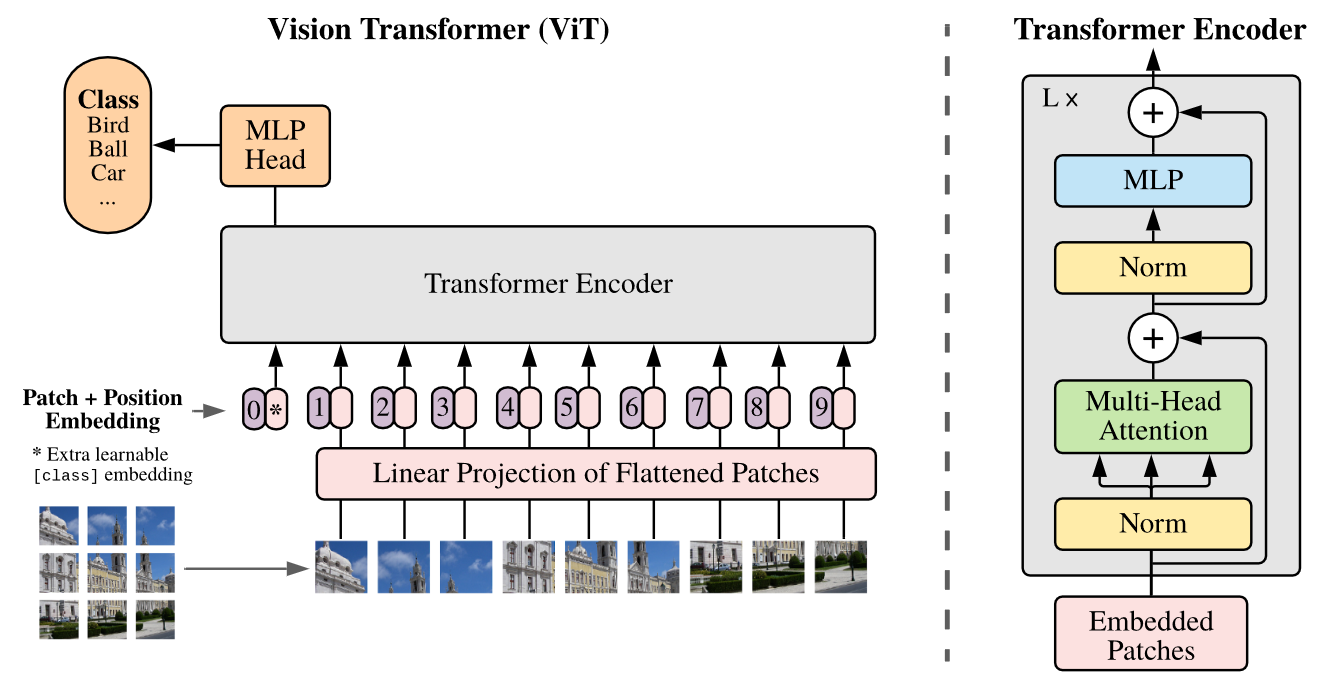
\includegraphics[width=0.95\linewidth]{vit.png}
%     %   \scriptsize Overview of Vision Transformer\\\parencite{dosovitskiyImageWorth16x162020}.
%     % \end{minipage}
%     \bottomleftrefs
%   \end{frame}
% \end{refsection}